\ifdefined\ishandout
\documentclass[11pt,handout]{beamer}
\else
\documentclass[11pt]{beamer}
\fi

% 日本語対応
\usepackage{luatexja}
\usepackage{luatexja-fontspec}
\renewcommand{\kanjifamilydefault}{\gtdefault}

\usepackage{mathptmx}
\renewcommand{\sfdefault}{lmss}
\renewcommand{\familydefault}{\sfdefault}
\usepackage[T1]{fontenc}
\usepackage{amsmath}
\usepackage{amssymb}
\usepackage{graphicx}
\PassOptionsToPackage{normalem}{ulem}
\usepackage{ulem}
\usepackage{caption}
\captionsetup{labelformat=empty}
\usepackage{bbm}
\usepackage{upgreek}
\setbeamertemplate{section in toc}[sections numbered]
\makeatletter
\usepackage{caption} 
\usepackage{bm}
\usepackage{subfig}
\captionsetup[table]{skip=10pt}
\usepackage{pdflscape}
\newcommand\makebeamertitle{\frame{\maketitle}}%
\AtBeginDocument{%
	\let\origtableofcontents=\tableofcontents
	\def\tableofcontents{\@ifnextchar[{\origtableofcontents}{\gobbletableofcontents}}
	\def\gobbletableofcontents#1{\origtableofcontents}
}

\def\Tiny{\fontsize{7pt}{8pt}\selectfont}
\def\Normal{\fontsize{8pt}{10pt}\selectfont}

\usetheme{Madrid}
\usecolortheme{lily}
\useinnertheme{rounded}

\setbeamertemplate{footline}{\hfill\Normal{\insertframenumber/\inserttotalframenumber}}
\setbeamertemplate{navigation symbols}{}

\newenvironment{changemargin}[2]{%
	\begin{list}{}{%
			\setlength{\topsep}{0pt}%
			\setlength{\leftmargin}{#1}%
			\setlength{\rightmargin}{#2}%
			\setlength{\listparindent}{\parindent}%
			\setlength{\itemindent}{\parindent}%
			\setlength{\parsep}{\parskip}% 
		}%
		\item[]}{\end{list}}

\setbeamertemplate{footline}{\hfill\insertframenumber/\inserttotalframenumber}
\setbeamertemplate{navigation symbols}{}

\usepackage{graphicx}
\usepackage{epsfig}
\usepackage{bm}
\usepackage{epsf}
\usepackage{float}
\usepackage[final]{pdfpages}
\usepackage{multirow}
\usepackage{colortbl}
\usepackage{xkeyval}
\usepackage{listings}
\usepackage{ifthen}
\usepackage{tikz}

\usepackage{xcolor,multirow,colortbl}
\usepackage{verbatim}
\usepackage{setspace}
\usepackage{ragged2e}

\setbeamersize{text margin left=1em,text margin right=1em} 

% Table formatting
\usepackage{booktabs}

% Decimal align
\usepackage{dcolumn}
\newcolumntype{d}[0]{D{.}{.}{5}}

\global\long\def\expec#1{\mathbb{E}\left[#1\right]}
\global\long\def\var#1{\mathrm{Var}\left[#1\right]}
\global\long\def\cov#1{\mathrm{Cov}\left[#1\right]}
\global\long\def\prob#1{\mathrm{Prob}\left[#1\right]}
\global\long\def\one{\mathbf{1}}
\global\long\def\diag{\operatorname{diag}}
\global\long\def\expe#1#2{\mathbb{E}_{#1}\left[#2\right]}
\DeclareMathOperator*{\plim}{\text{plim}}

\usepackage{appendixnumberbeamer}
\renewcommand{\thefootnote}{}

\setbeamertemplate{footline}
{
	\leavevmode%
\hfill
	\insertframenumber{}\hspace*{2ex}\vspace{1ex}
}

\makeatother

\usepackage[english]{babel}

\usepackage{tikz}
\newcommand*\circled[1]{\tikz[baseline=(char.base)]{             \node[circle,ball color=structure.fg, shade,   color=white,inner sep=1.2pt] (char) {\tiny #1};}} 

\makeatletter
\let\save@measuring@true\measuring@true
\def\measuring@true{%
	\save@measuring@true
	\def\beamer@sortzero##1{\beamer@ifnextcharospec{\beamer@sortzeroread{##1}}{}}%
	\def\beamer@sortzeroread##1<##2>{}%
	\def\beamer@finalnospec{}%
}
\makeatother

\setbeamersize{text margin left= .8em,text margin right=1em} 
\newenvironment{wideitemize}{\itemize\addtolength{\itemsep}{10pt}}{\enditemize}
\newenvironment{wideitemizeshort}{\itemize}{\enditemize}

\newcommand{\indep}{\perp\!\!\!\!\perp} 

\DeclareMathOperator*{\argmax}{arg\,max}
\DeclareMathOperator*{\argmin}{arg\,min}

\begin{document}
	
	%% タイトルスライド
	\begin{frame}[noframenumbering]{}
		\vspace{0.5cm}
		\title[]{第8章：回帰不連続デザイン}
		\author{Jonathan Roth}
		\date{数理計量経済学 I \\ ブラウン大学\\} 
		\titlepage {\small{}\ }\thispagestyle{empty} \vspace{-30pt}
		
	\end{frame}

	
	\begin{frame}{モチベーション}
		
		\vspace{0.1cm}
		\begin{wideitemizeshort}
			\item
			因果推論における主要な課題は、処置ステータス以外はあらゆる面で処置群と比較可能な対照群を見つけることです。\pause{}
			
			\item
			これまで、以下のような場合に因果的効果を推定する方法を見てきました：\smallskip\pause{}
			\begin{itemize}
			\item 処置が文字通りランダムに割り当てられている場合\smallskip\pause{}
			\item 処置が実質的にランダムに割り当てられている場合（条件付き非交絡性）\smallskip\pause{}
			\item 選択バイアスが時間を通じて一定である場合（並行トレンド）\smallskip\pause{}
			\item 実質的にランダムで除外制約を満たす操作変数がある場合
			\end{itemize} 
						
			\pause
			\item
			本日は、もう一つの戦略である\textbf{回帰不連続デザイン (RD)} を見ていきます。
			
			\pause			
			\item
			RD の背後にある考え方は、スコアがしきい値を上回るか下回るかによって、処置ステータスが決定される場合があるということです。
			\pause\smallskip
				\begin{itemize}
					\item 
					例えば、学校への入学が、テストの点数があるカットオフ値を超えるかどうかに依存する場合などです。
				\end{itemize} 
			
			\pause
			\item
			このような場合、RD はスコアがしきい値を「わずかに」上回る人々と、下回る人々の結果を比較します。
		\end{wideitemizeshort}
		
	\end{frame}


	\begin{frame}{例：Hu and Chao (2008)}
		\begin{wideitemize}
			\item
			Hu and Chao (2008) は以下の問いに興味を持っています：健康保険の欠如は、貧困層が重要な医療を受けることを妨げているか？
			
			\pause
			\item
			単に健康保険がある人とない人の医療利用を比較するだけではいけないのはなぜでしょうか？
			\pause
				\begin{itemize}
					\item 
					交絡変数があるからです！ 健康保険を持っている人はより裕福である可能性があり、それが直接健康状態に影響を与えているかもしれません。
				\end{itemize}
			
			\pause
			\item
			背景：グルジア共和国（米国のジョージア州ではありません！）は2006年に健康保険プログラムを創設しました。各世帯は80の変数から導出された「貧困スコア」を付与され、スコアが100,000\textbf{以下}の世帯が健康保険を受け取りました。
			
			\pause
			\item
			鍵となるアイデア：スコアが100,000をわずかに上回る世帯は、100,000をわずかに下回る世帯と非常に似ているはずです。\smallskip\pause{}
			\begin{itemize}
			\item 唯一の違いは、100,000以下の世帯が健康保険という「処置」を受けたことです！
			\end{itemize}
		\end{wideitemize}
	\end{frame}
	
	\begin{frame}
		\centering
		\includegraphics[width = 0.7\linewidth]{hou-rdd-basic}
		\begin{wideitemize}
			\item
			このプロットは、スコアの関数としての結果（急激な手術の件数）を示しています。
		\end{wideitemize}	
	\end{frame}

	\begin{frame}
	\centering
	\includegraphics[width = 0.7\linewidth]{hou-rdd-eligibility}
	\begin{wideitemize}
		\item
		垂直線（100,000）の左側のグループが政府から健康保険を受け取ります。
		
		\item
		100,000をわずかに下回る人々と、わずかに上回る人々は、保険の受給資格以外のすべての要因において非常に似ていることが期待されます。
	\end{wideitemize}	
\end{frame}

	\begin{frame}
	\centering
	\includegraphics[width = 0.7\linewidth]{hou-rdd-means}
	\begin{wideitemize}
		\item
		100,000をわずかに下回る人々と、わずかに上回る人々は、保険の受給資格以外のすべての要因において非常に似ていることが期待されます。
		
		\item
		しかし、しきい値のすぐ左側の人々は、右側の人々よりも明らかに多く手術を受けているようです！
	\end{wideitemize}	
\end{frame}

	\begin{frame}
	\centering
	\includegraphics[width = 0.7\linewidth]{hou-rdd-treatment-effect}
	\begin{wideitemize}		
		\item
		しかし、しきい値のすぐ左側の人々は、右側の人々よりも明らかに多く手術を受けているようです！
		
		\item
		もし他のすべての要因がしきい値において連続的であれば、この差が（しきい値付近の人々における）因果的効果となります！
	\end{wideitemize}	
\end{frame}

\begin{frame}{RD の定式化}
	\begin{wideitemizeshort}
		\item
		$D_i$ を処置のバイナリ指標、\pause $R_i$ を\textbf{実行変数} (running variable) とします。
		
		\pause
		\item
		\textbf{シャープな} (sharp) RD では、ユニット $i$ は $R_i \geq c$ の場合にのみ処置を受けます：
		$$D_i = 1[ R_i \geq c ] $$
		
		\pause\smallskip
		\begin{itemize}
		\item $D_i$ は交絡因子の可能性が高い変数によって\textbf{決定論的}に決まります。
		\end{itemize}
		\item 
		RD の考え方は、カットオフ $c$ の周囲における CEF の極限を比較することです：
		
		$$\tau_{RD} = \underbrace{ \lim_{r \downarrow c} E[Y_{i} | R_i = r] }_{\text{上からの極限} }- \underbrace{\lim_{r \uparrow c} E[Y_{i} | R_i = r]}_{\text{下からの極限} } $$
		

		\pause
		\item 
		どのような場合に $\tau_{RD}$ が因果的効果に対応するのでしょうか？ 
	\end{wideitemizeshort}
\end{frame}

\begin{frame}{極限を考える}
\begin{wideitemizeshort}
	\item
	$R_i < c$ の人々は $D_i = 0$ です。したがって：
	$\lim_{r \uparrow c} E[Y_{i} | R_i = r] = \pause{}  \lim_{r \uparrow c} E[Y_{i}(0) | R_i = r]$
	
	\pause
	\item 
	$R_i \geq c$ の人々は $D_i = 1$ です。したがって：
	$\lim_{r \downarrow c} E[Y_{i} | R_i = r] = \pause{} \lim_{r \downarrow c} E[Y_{i}(1) | R_i = r]$
	
	\pause
	\item
	\textbf{仮定：} $E[Y_{i}(d) | R_i = r]$ が $d= 0,1$ について $c$ で\textbf{連続}ならば：
	\smallskip\pause{}
	\begin{itemize}
	\item $\lim_{r \uparrow c} E[Y_{i}(0) | R_i = r]=E[Y_{i}(0) | R_i = c]$\smallskip\pause{}
	\item $\lim_{r \downarrow c} E[Y_{i}(1) | R_i = r]=E[Y_{i}(1) | R_i = c]$
	\end{itemize}
	\pause
	\item
	したがって：
	{\small $$\tau_{RD} =\lim_{r \downarrow c} E[Y_{i}(1) | R_i = r]- \lim_{r \uparrow c} E[Y_{i}(0) | R_i = r] = E [Y_{i}(1) - Y_{i}(0) | R_i = c] $$}
	\pause これは、カットオフ地点における平均処置効果です！
\end{wideitemizeshort}

\end{frame} 


\begin{frame}{連続性の評価}
	\begin{wideitemize}
		\item
		RD における最も重要な仮定は、潜在的結果の期待値 $E[Y_i(d) | R_i = r]$ がカットオフにおいて連続である（ $d=0,1$ について）ことです。
		
		\pause
		\item
		なぜ連続性の仮定が満たされない可能性があるのでしょうか？
		
		\pause
		\item
		理由1：交絡因子がカットオフにおいて不連続に変化する場合。
		
		\pause
		\item
		理由2：人々がカットオフの直上/直下に入るようにスコアを\textbf{操作} (manipulate) できる場合。
		
	\end{wideitemize}
\end{frame}	

\begin{frame}{例：交絡因子}
	\begin{wideitemize}
		\item
		政策はしばしば州境において不連続に変化します。
		
		\pause
		\item
		例：Holmes (1998) は、労働組合を弱める「労働権法 (right-to-work laws)」がビジネスにどのように影響するかに興味を持っています。
		
		\pause
		\item
		彼は RD を用いて、労働権法がある州とない州の境界の両側で、製造業の雇用密度を比較しました。
	\end{wideitemize}
\end{frame}
	
	
\begin{frame}
\begin{center}
\includegraphics[width = 0.55\linewidth]{rtw-figure-2}\\
\includegraphics[width = 0.55\linewidth]{rtw-figure-1}	
\end{center}
\end{frame}	

\begin{frame}
\begin{center}
	\includegraphics[width = 0.75 \linewidth]{rtw-results}
\end{center}
	\begin{wideitemize}
		\item
		境界線の労働権法（RTW）がある側で、製造業が多いように見えます。
		
		\pause
		\item
		しかし、州境で変化するのは労働権法だけでしょうか？！ 労働権法が、製造業に影響を与える他の政策と相関している可能性はないでしょうか？
	\end{wideitemize}
\end{frame}

\begin{frame}
	\begin{wideitemize}
		\item
		このような懸念に部分的に対処するため、観察可能な特徴がカットオフにおいて不連続に変化していないことを示すのが一般的です。
		
		\pause
		\item
		下の図は、Hou and Chao の論文において、年齢、性別、教育、世帯人数に不連続性が見られないことを示しています。
		
	\end{wideitemize}	
	\centering
	\includegraphics[width = 0.7 \linewidth]{hou-balance}

	\pause
	\begin{wideitemize}
		\item
		しかし、いつものように、他の未観察の交絡因子がカットオフにおいて変化している可能性は依然として残ります。
	\end{wideitemize}
\end{frame}

\begin{frame}{例：操作}
	\begin{wideitemizeshort}
		\item
		ニューヨーク市では、高校卒業資格を得るために Regents 試験で少なくとも55点を取る必要があります。
		
		\pause
		\item
		これを利用した卒業資格の効果の研究は魅力的ですが... 実際には、しきい値のすぐ上に非常に多くの生徒が集中しています。
		\begin{center}
		\includegraphics[width = 0.45 \linewidth]{regents-discontinuity}
		\end{center}
		
		\pause
		\item
		考えられる理由：教師が、生徒をしきい値に乗せるために「おまけ」をしている可能性があります。
		
		\pause
		\item
		しきい値をギリギリ超えた生徒と、そうでない生徒が似ているとは言えません。
	\end{wideitemizeshort}
\end{frame}

\begin{frame}{操作のテスト}
	\begin{wideitemize}
		\item
		このような RD の操作をテストするために、カットオフの両側でユニットの数が同様であるかを確認するのが一般的です。これはしばしば「マクレアリー・テスト (McCrary test)」と呼ばれます。
		
		\item
		カットオフの片側に「集積 (bunching)」が見られる場合、通常は操作の証拠として解釈されます。
		
		\item
		集積がある場合、連続性の仮定は非常に疑わしいものになります。
	\end{wideitemize}
\end{frame}

	
	
\begin{frame}{RD の推定}
	\begin{itemize}
		\item 
		連続性の下で、識別式は以下の通りです：
		$$\lim_{r \downarrow c} E[Y_{i} | R_i = r] - \lim_{r \uparrow c} E[Y_{i} | R_i = r]= E[Y_i(1)-Y_i(0)\mid R_i=c]$$ 
		
		\pause
		\item
		この CATE を推定するには、実行変数 $R_i$ が与えられたときのアウトカム $Y_i$ の CEF を推定し、極限をとるだけです。\bigskip
		
		\pause
		\item
		CEF を推定するには？ \pause{} OLS です！
	\end{itemize}
\end{frame}

\begin{frame}{線形回帰を用いた RD}
	\begin{wideitemize}
		\item
		CEF が区分的に線形であると仮定しましょう：
		\begin{align*}
			& E[Y_i | R_i = r] \approx \alpha_0 + \alpha_1 r  \hspace{2cm} \text{ if } r <c \\
			& E[Y_i | R_i = r] \approx \beta_0 + \beta_1 r \hspace{2cm} \text{ if }  r \geq c
		\end{align*}
	
	\pause
	\item
	すると RD の仮定の下で：
	$$CATE = \lim_{r \downarrow c} E[Y_{i} | R_i = r] - \lim_{r \uparrow c} E[Y_{i} | R_i = r] \approx \pause{} (\beta_0 + \beta_1 c) - (\alpha_0 + \alpha_1 c) $$
	\pause
	\item
	これらの回帰係数を OLS で推定することで、処置の効果を推定できます。
	\end{wideitemize}
\end{frame}

\begin{frame}{1つの回帰で実行する}
	\begin{wideitemize}
		\item
		一般性を失うことなく $c=0$ と正規化すれば、実は1つの回帰でこれを行うことができます。
		
		\pause
		\item
		以下の回帰を考えます：
		\begin{align*}
			Y_i  = \alpha +  \beta 1[R_i \geq 0]  + \gamma R_i  + \delta  R_i 1[R_i \geq 0 ]  + U_i
		\end{align*}
		
		\pause
		\item
		すると：
		\begin{align*}
			  \text{ if } r <0, \hspace{2cm} E[Y_i | R_i = r] \approx & \pause{} \alpha + \gamma r   \\ \pause{}
			 \text{ if }  r \geq 0, \hspace{2cm} E[Y_i | R_i = r] \approx & \pause{} \alpha + \beta  + \gamma r + \delta r 
		\end{align*}
		 
		\pause
		\item
		したがって：
		\begin{align*}
			ATE& = \lim_{r \downarrow 0} E[Y_{i} | R_i = r] - \lim_{r \uparrow 0} E[Y_{i} | R_i = r] \\
			&\approx \pause{} (\alpha  + \beta + (\gamma + \delta) \times 0 ) - (\alpha + \gamma \times 0 ) = \pause{} \beta 
		\end{align*} 
	\end{wideitemize}
\end{frame}

\begin{frame}
\vspace{0.2cm}
	\centering
	\includegraphics[width = 0.9 \linewidth]{rd_linear2}
\end{frame}


\begin{frame}{高次の項}
	\begin{wideitemizeshort}
		\item
		これは、CEF への線形近似が適切である場合にのみうまく機能します。
		
		\pause
		\item
		これまでと同様に、回帰に高次の項を加えることもできます。
		
		\pause
		\item
		例えば、ここでは両側で2次式をフィットさせています：
		\begin{center}
		\includegraphics[width = 0.65\linewidth]{rd_quad}
		\end{center}
		
	\end{wideitemizeshort}
\end{frame}

\begin{frame}{高次多項式の問題点}
	\begin{wideitemize}
		\item
		高次多項式の問題は、データに過剰適合（過学習）してしまう可能性があることです。
			\begin{wideitemize}
				\item
				特に、データの「境界」に向かって外挿する際に、この問題は深刻になります。
			\end{wideitemize}
		
		\pause
		\item
		この図の中に、本当に不連続性は存在しますか？ 
		\begin{center}
		\includegraphics[width = 0.7 \linewidth]{rd-over-fitting}
		\end{center}
	\end{wideitemize}
\end{frame}

\begin{frame}{線形に固執すべきか？}
	過学習の問題により、あるノーベル賞受賞者（かつブラウン大卒業生）は強い立場をとっています！ \vspace{1cm}
	\begin{center}
	\includegraphics[width = 0.7 \linewidth]{gelman-imbens}
	\end{center}
\end{frame}

\begin{frame}{実務ではどうすればよいか？}
	\begin{wideitemize}
		\item
		明らかに、CEF を十分に捉える豊かな近似と、過学習との間にはトレードオフがあります。
		
		\pause
		\item
		実務における標準的なアプローチは、\textbf{局所線形回帰} (local linear regression) を用いることです。
		
		\pause
		\item
		基本的な考え方は、線形回帰をフィットさせますが、境界に「近い」点のみを使用することです。
		
				\pause
				\begin{itemize}
					\item 
					最も単純なケースでは、カットオフの「バンド幅 (bandwidth)」内の点のみを使用します。
					
					\pause
					\item
					より複雑なバージョンでは、カットオフに近い観測値ほど高い重みを付けます。
				\end{itemize}
			
		\pause
		\item
		バンド幅を選ぶためのデータ駆動型の方法もいくつかあります（例：観測値が多い場合はより狭いバンド幅を使う）。
		
		\pause
		\item
		これは Stata の \texttt{rd} パッケージなどを用いることで、簡単に実装できます。
	\end{wideitemize}
\end{frame}

\begin{frame}{局所線形回帰}
	\begin{center}
	\includegraphics[width = 0.8 \linewidth]{rd_llin}
	\end{center}
\end{frame}

\begin{frame}{RD の推定は難しい！}
	\begin{wideitemize}
		\item
		局所線形回帰は、モデルの豊かさと過学習の間の比較的良い妥協点です。
		
		\item
		しかし、完璧ではありません！ 一般に、非常に非線形な CEF と不連続性を区別するのは困難です。
		
		\pause
		\item
		自分の目を信じることも大切です。プロットを見て、不連続性があるように見えますか？
		

		\item
		最も説得力のある RD は、プロットから一目瞭然であり、高度な計量経済学的手法を必要としません。
	\end{wideitemize}
\end{frame}

%\begin{frame}{Looks Can Be Deceiving!}
%	\begin{center}
%	\includegraphics[width = 0.8 \linewidth]{rd_truth}
%	\end{center}
%\end{frame}

	
	
\begin{frame}{ファジーな RD}
	\begin{wideitemize}
		\item
		しきい値を超えることが、処置ステータスを完全には決定しないこともあります。しかし、処置を受ける確率が不連続に上昇する場合があります。
		
		\item
		これは\textbf{ファジーな} (fuzzy) RD と呼ばれます。
		
		\pause
		\item
		基本的な考え方は IV と似ています。しきい値を超えることがアウトカムに与える効果を推定し、それを処置ステータスへの効果（すなわち処置確率の変化）で割ります。
		
		\pause
		\item
		特定の条件下で、これはカットオフ地点における LATE を識別します。
	\end{wideitemize}
\end{frame}

\begin{frame}{例：Bleemer and Mehta (2022)}
	\begin{wideitemize}
		\item
		Bleemer and Mehta は、（皆さんにとって）非常に重要な問いを投げかけています：経済学を専攻するとお金持ちになれるのか？
		
		\pause
		\item
		彼らはこの問題をカリフォルニア大学サンタクルーズ校 (UCSC) の文脈で研究しました。そこでは経済学部が、入門科目の GPA が 2.8 未満の学生に対し、経済学専攻を「学部の裁量」として制限していました。
	\end{wideitemize}
\end{frame}

\begin{frame}{第一段階}
	\centering
	\includegraphics[width = 0.7 \linewidth]{bleemer-first-stage}
	
	しきい値を超えた学生は、経済学を専攻する確率が約 36 ポイント高くなっています。
\end{frame}

\begin{frame}
	\centering
	\includegraphics[width= 0.7 \linewidth]{bleemer-rf}
	
	\begin{wideitemize}
		\item
		しきい値を超えた学生は、所得が約 8,000 ドル多くなっています。
		
		\pause
		\item
		この講義を履修してよかったと思いませんか？！
		
		\pause
		\item
		経済学専攻の効果のファジー RD 推定値は、 \$8,000 / 0.36 $\approx$ \$22,000 となり、これは平均所得の 40% に相当します。
	\end{wideitemize}
\end{frame}	

\begin{frame}{どのような場合にファジー RD は LATE を与えるか？}
	\begin{wideitemize}
		\item
		IV と同様の仮定の下で、ファジー RD はカットオフ地点におけるコンプライヤーの LATE を与えます。
		
		\pause
		\item
		\textbf{連続性}。 $d=0,1$ について $E[Y_i(d) | R_i]$ がカットオフで連続であること。また、コンプライヤー/オールウェイズ・テイカー/ネバー・テイカーの割合も連続である必要があります。
		
		
		\item
		\textbf{除外制約}。カットオフの直上/直下であることは、処置ステータスへの影響を通じてのみアウトカムに影響を与えること。
		
		
		\item \textbf{関連性}。カットオフにおいて処置の受け入れに不連続性が存在すること。
		
		
		\item \textbf{「局所的」単調性}。カットオフを下回る場合にのみ処置を受ける、というディファイアーが存在しないこと。
	\end{wideitemize}
\end{frame}


\begin{frame}{Dell and Querubin (2017)}
\begin{wideitemize}
	\item
	Dell and Querubin は、ベトナム戦争中に米国空軍が、村の169の治安・政治・経済的特徴に基づいた「リスクスコア」を用いて爆撃目標を選定していた事実を利用しました。
	
	\item
	アルゴリズムは連続的なスコアを算出しましたが、将軍たちに渡される前に最も近い整数に四捨五入されていました。 $\rightarrow$ Dell and Querubin は、この四捨五入による不連続性を利用しました。
\end{wideitemize}	
\centering 
\includegraphics[width = 0.5\linewidth]{dell-first-stage}
\end{frame}

\begin{frame}{バランスの確認}
	\begin{wideitemizeshort}
		\item
		しきい値の直上と直下の地域は、爆撃の決定が行われる前は同様の特徴を持っていました。
		
		\item
		例えば、そのスコアが使われるようになる前の爆撃回数は同様でした。
	\end{wideitemizeshort}

\centering 
\includegraphics[width = 0.65\linewidth]{dell-balance}
\end{frame}

\begin{frame}

\begin{wideitemize}
	\item
	爆撃は村々にとって悪影響だったようです $\rightarrow$ 学校の数が減少しました。
\end{wideitemize}

\centering 
\includegraphics[width = 0.7\linewidth]{dell-schools}	
\end{frame}

\begin{frame}
	
	\begin{wideitemize}
		\item
		爆撃は軍事目標にとっても悪影響だったようです $\rightarrow$ 長期的なベトコン (VC) の活動が活発化しました。
	\end{wideitemize}
	
	\centering 
	\includegraphics[width = 0.7\linewidth]{dell-vc}	
\end{frame}

\begin{frame}{結論として...}
	\begin{wideitemize}
		\item
		爆撃は良くない $\checkmark$
		
		\item
		計量経済学は良い $\checkmark$
		
	\end{wideitemize}
\end{frame}

\begin{frame}{Zimmerman (2009)}
	\begin{wideitemizeshort}
		\item
		Zimmerman (2009) は、4年制の州立大学に通うことの所得への影響を研究しました。
		
		\item
		フロリダ州立大学の中で最も選択度の低いフロリダ国際大学 (FIU) に焦点を当てました。
		
		\item
		州法は州立大学の学生に少なくとも 3.0 の GPA を求めていましたが、FIU は計算方法が最も寛大でした。
		
		\item
		したがって、FIU のしきい値付近にいる学生は、通常、フロリダの他のどの4年制公立大学の資格も持っていませんでした。
		
		\item
		Zimmerman は、3.0 の GPA カットオフを用いたファジー RD デザインを行いました。
	\end{wideitemizeshort}
\end{frame}

\begin{frame}
	\centering
	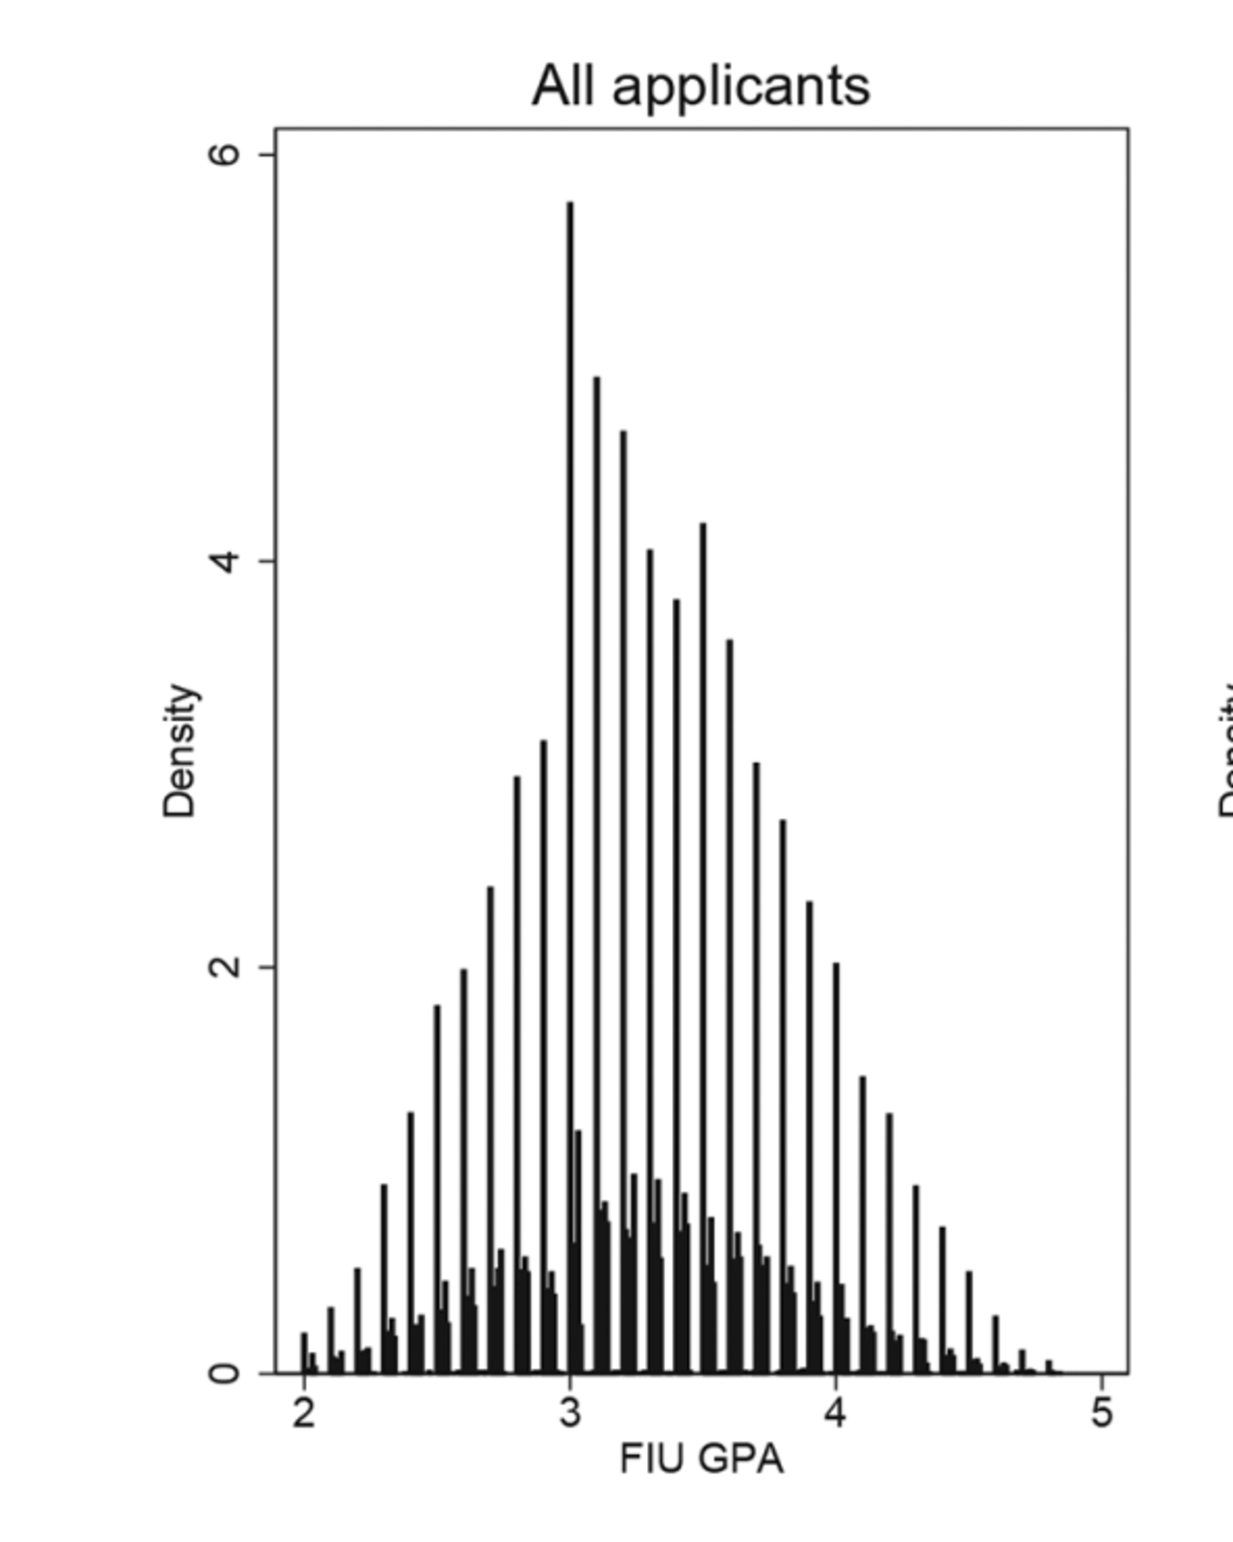
\includegraphics[width = 0.5\linewidth]{zimmerman-bunching}
	
	一つの懸念：カットオフの直上に集積が見られます。意欲の高い学生が、必要な GPA を\textbf{ぴったり}取るように調整したのでしょうか？ \medskip
	
	あるいは、2.99 よりも 3.0 になる成績の組み合わせの方が多いのかもしれません。
\end{frame}

\begin{frame}
	\centering
	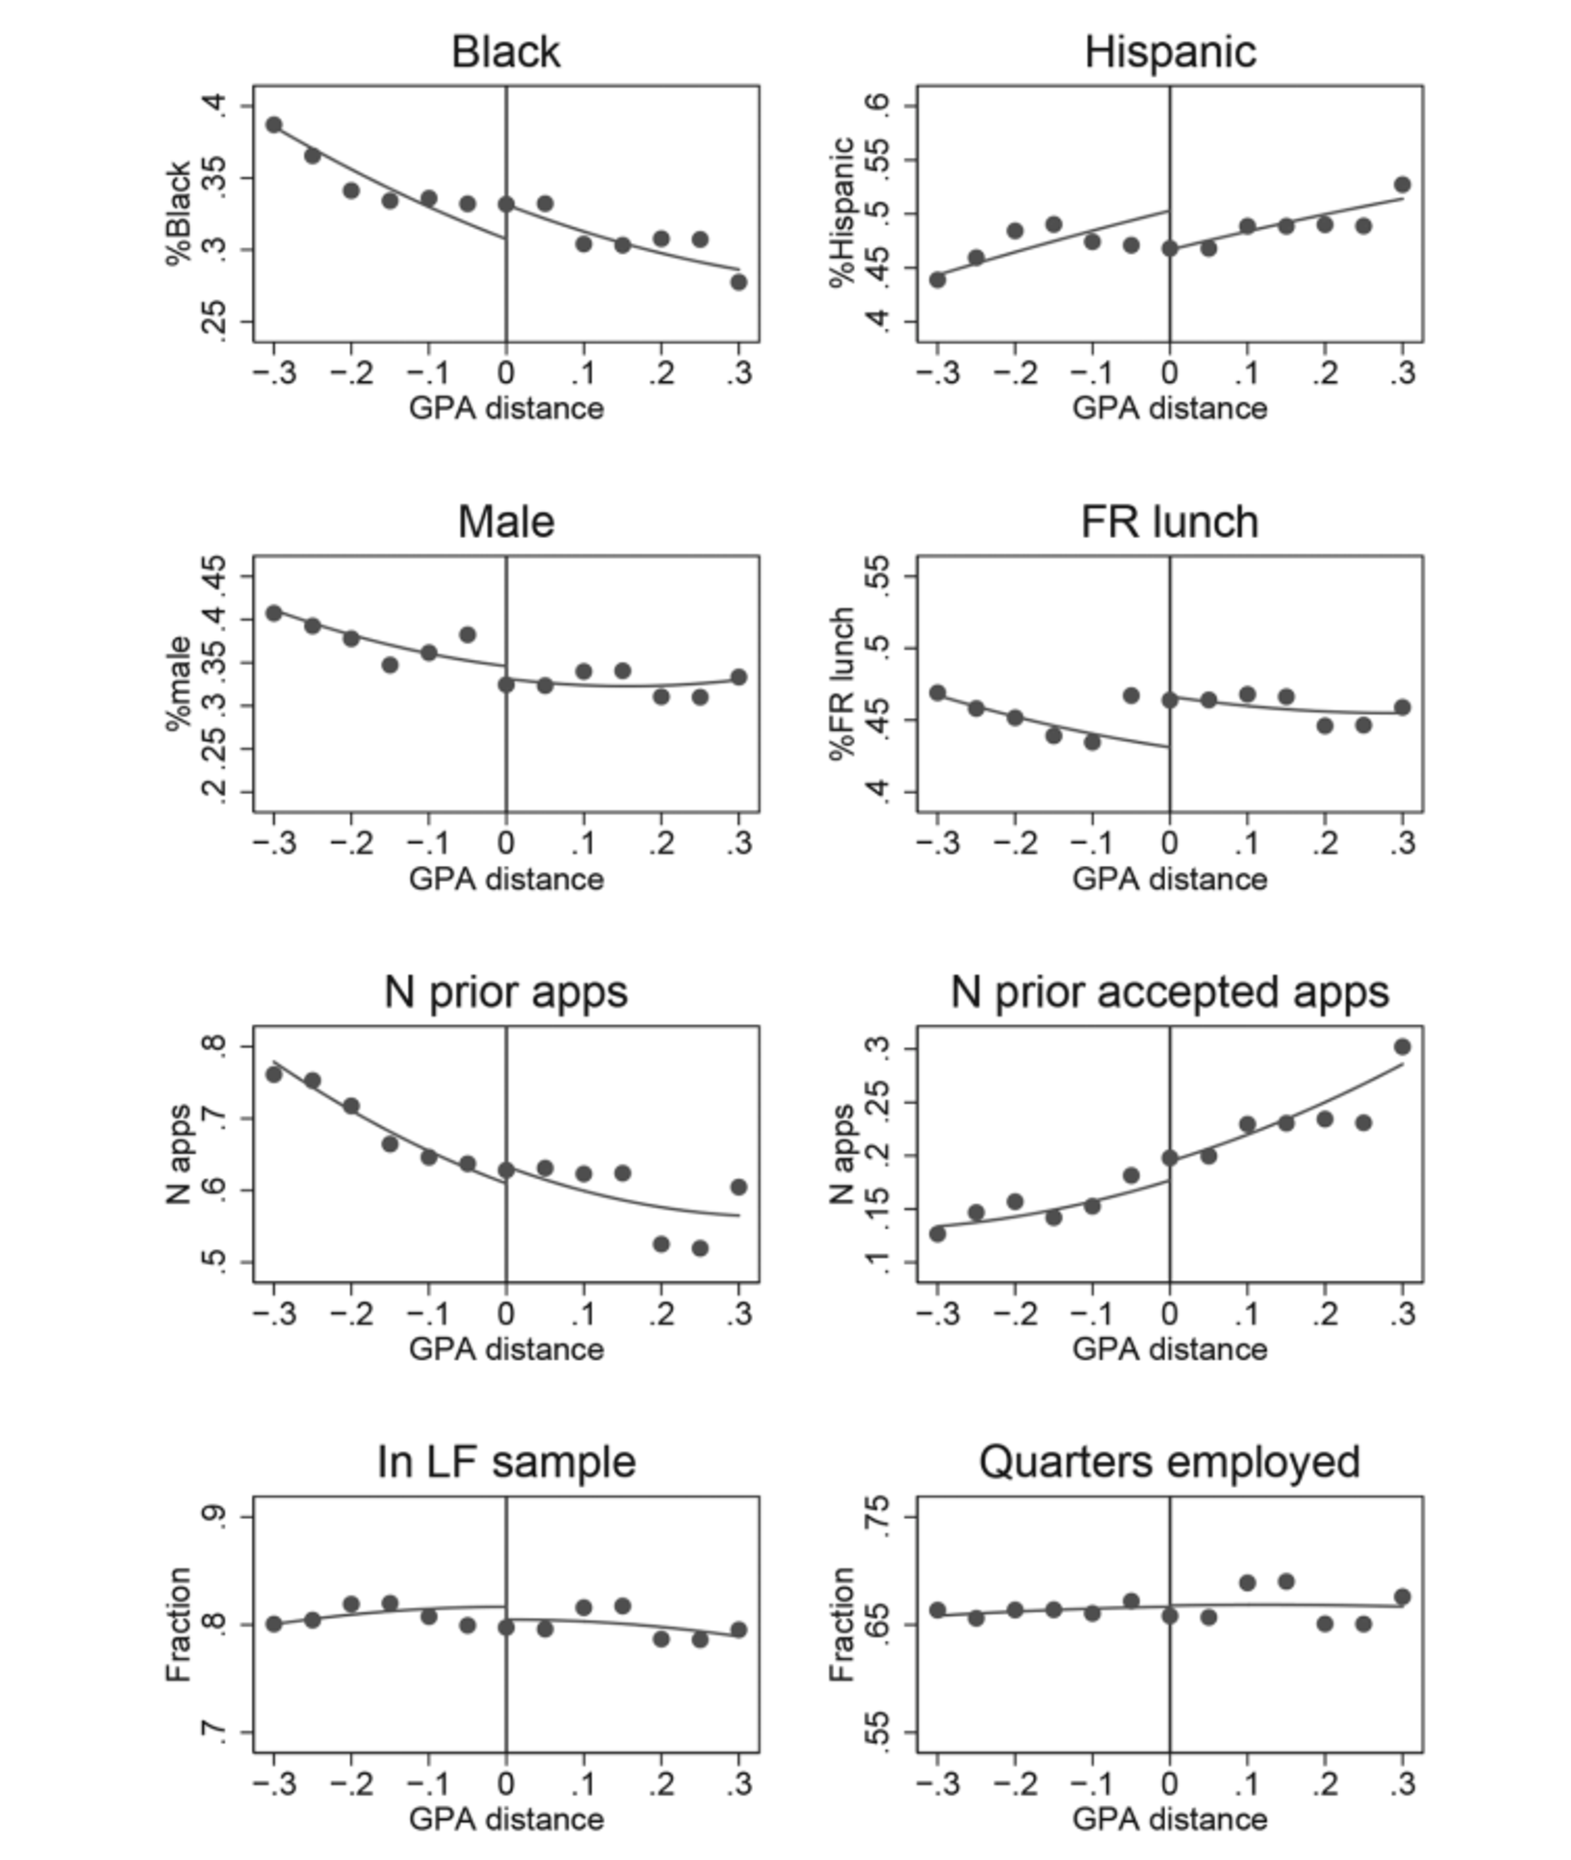
\includegraphics[width = 0.5 \linewidth]{zimmerman-balance}
	
	
	しかし、カットオフ周辺で観察可能な特徴に不連続性は見られません。
\end{frame}

\begin{frame}{第一段階}
\centering
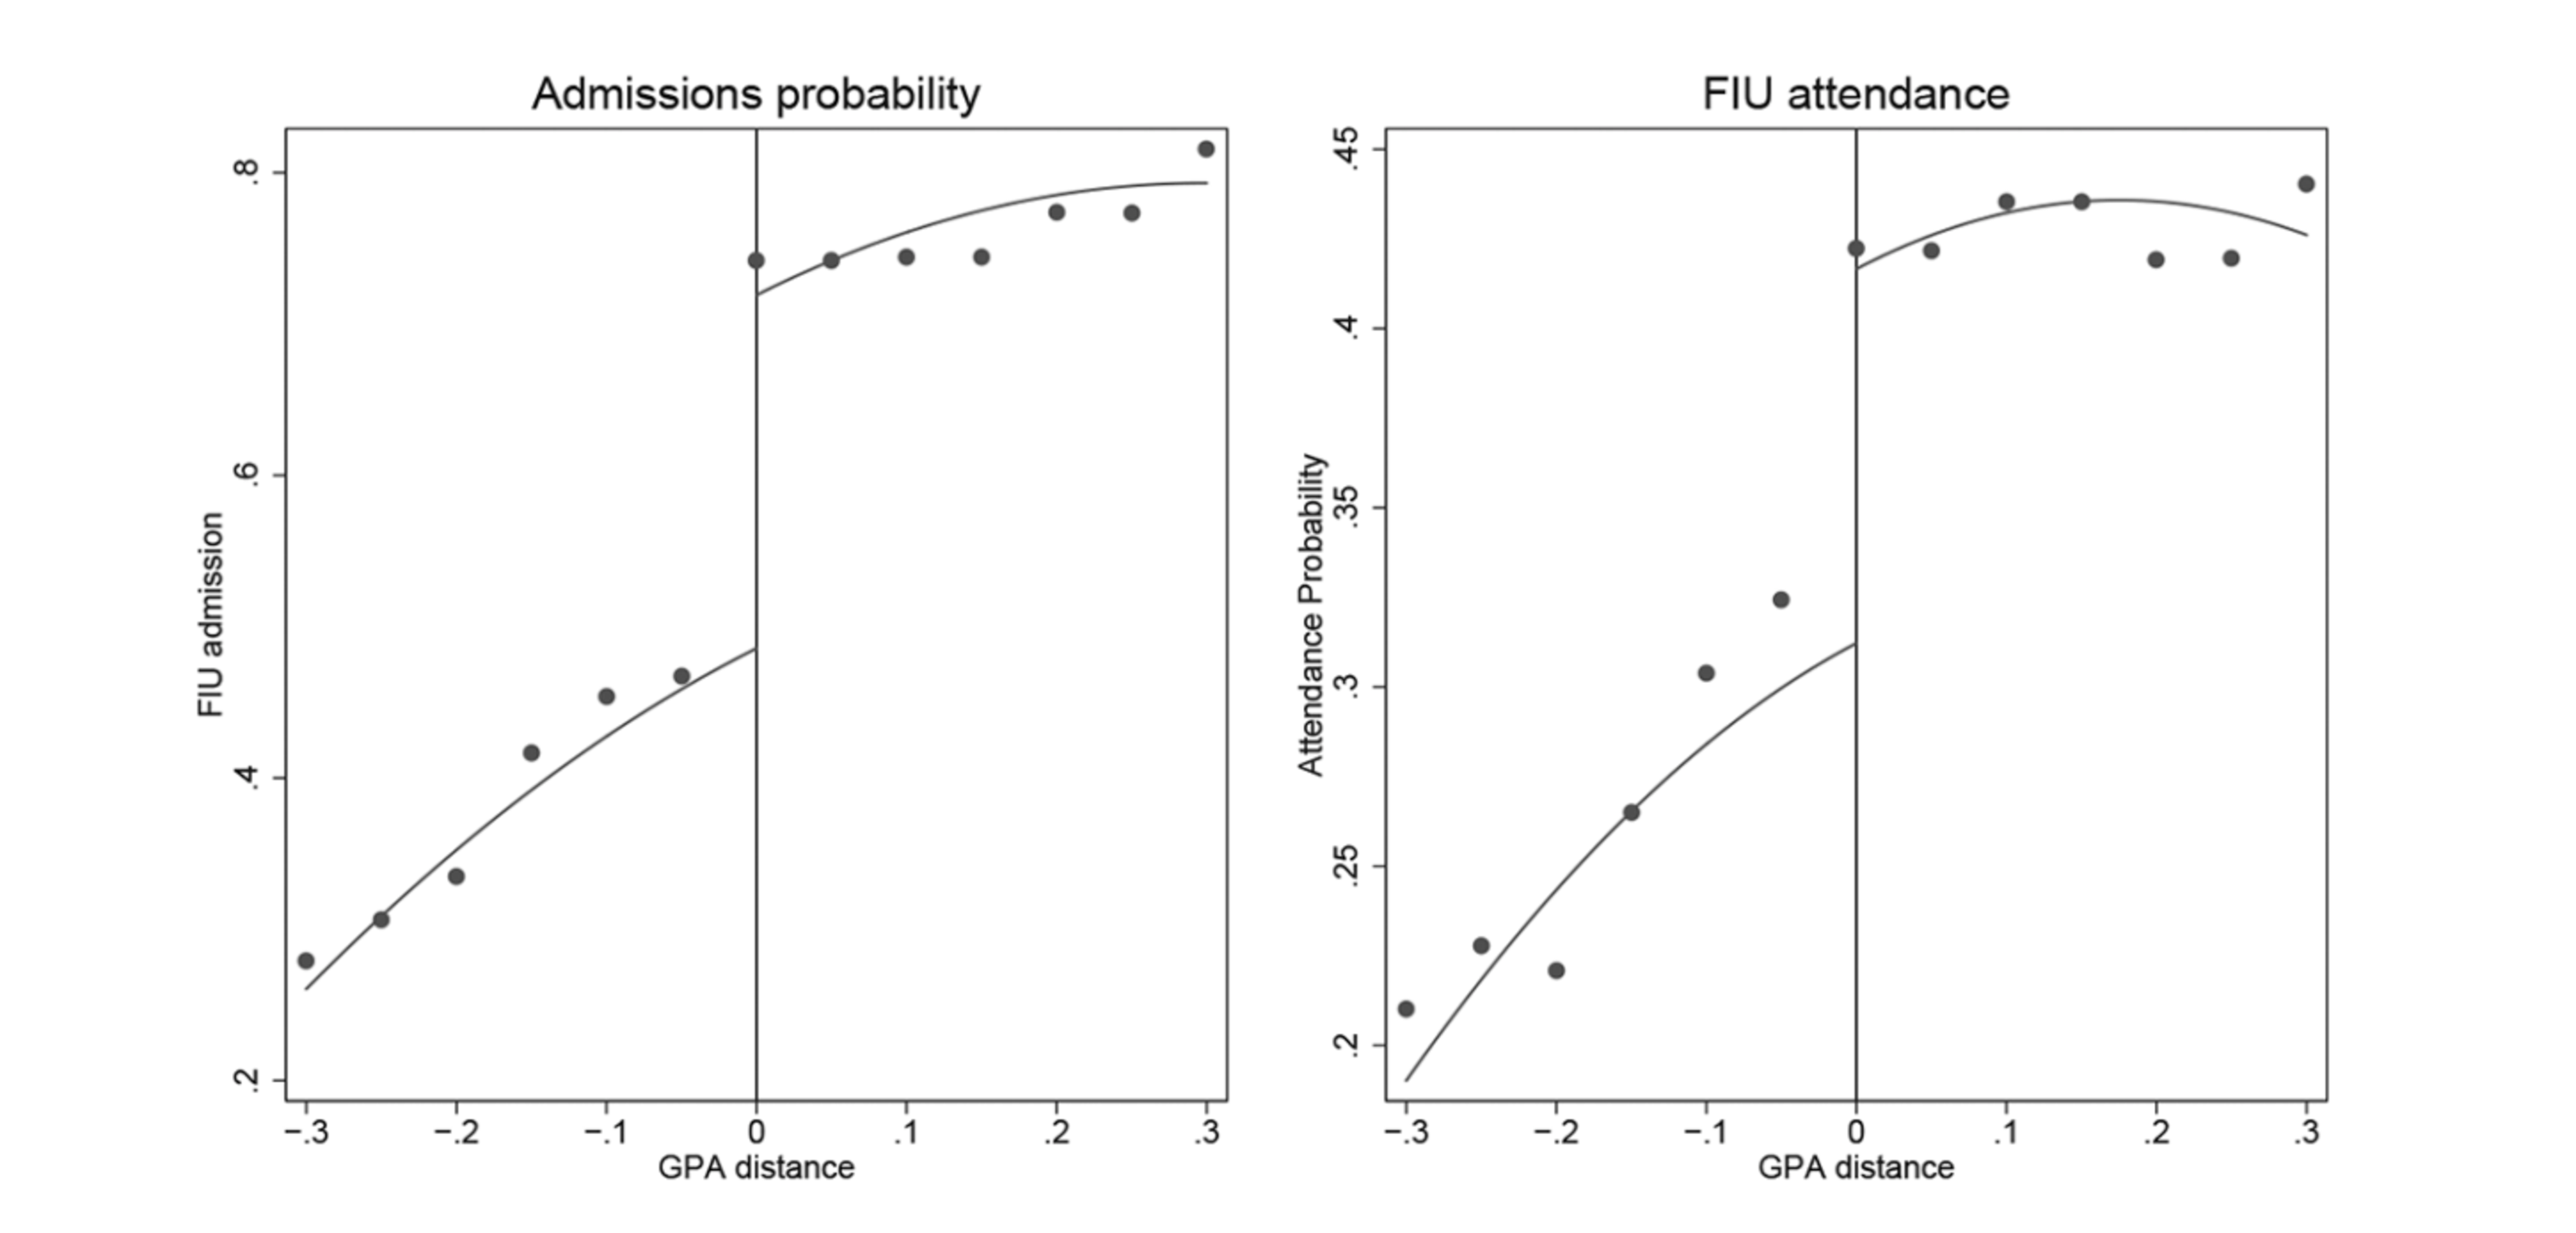
\includegraphics[width = 0.8 \linewidth]{zimmerman-fs}
\end{frame}

\begin{frame}{誘導型}
	\centering
	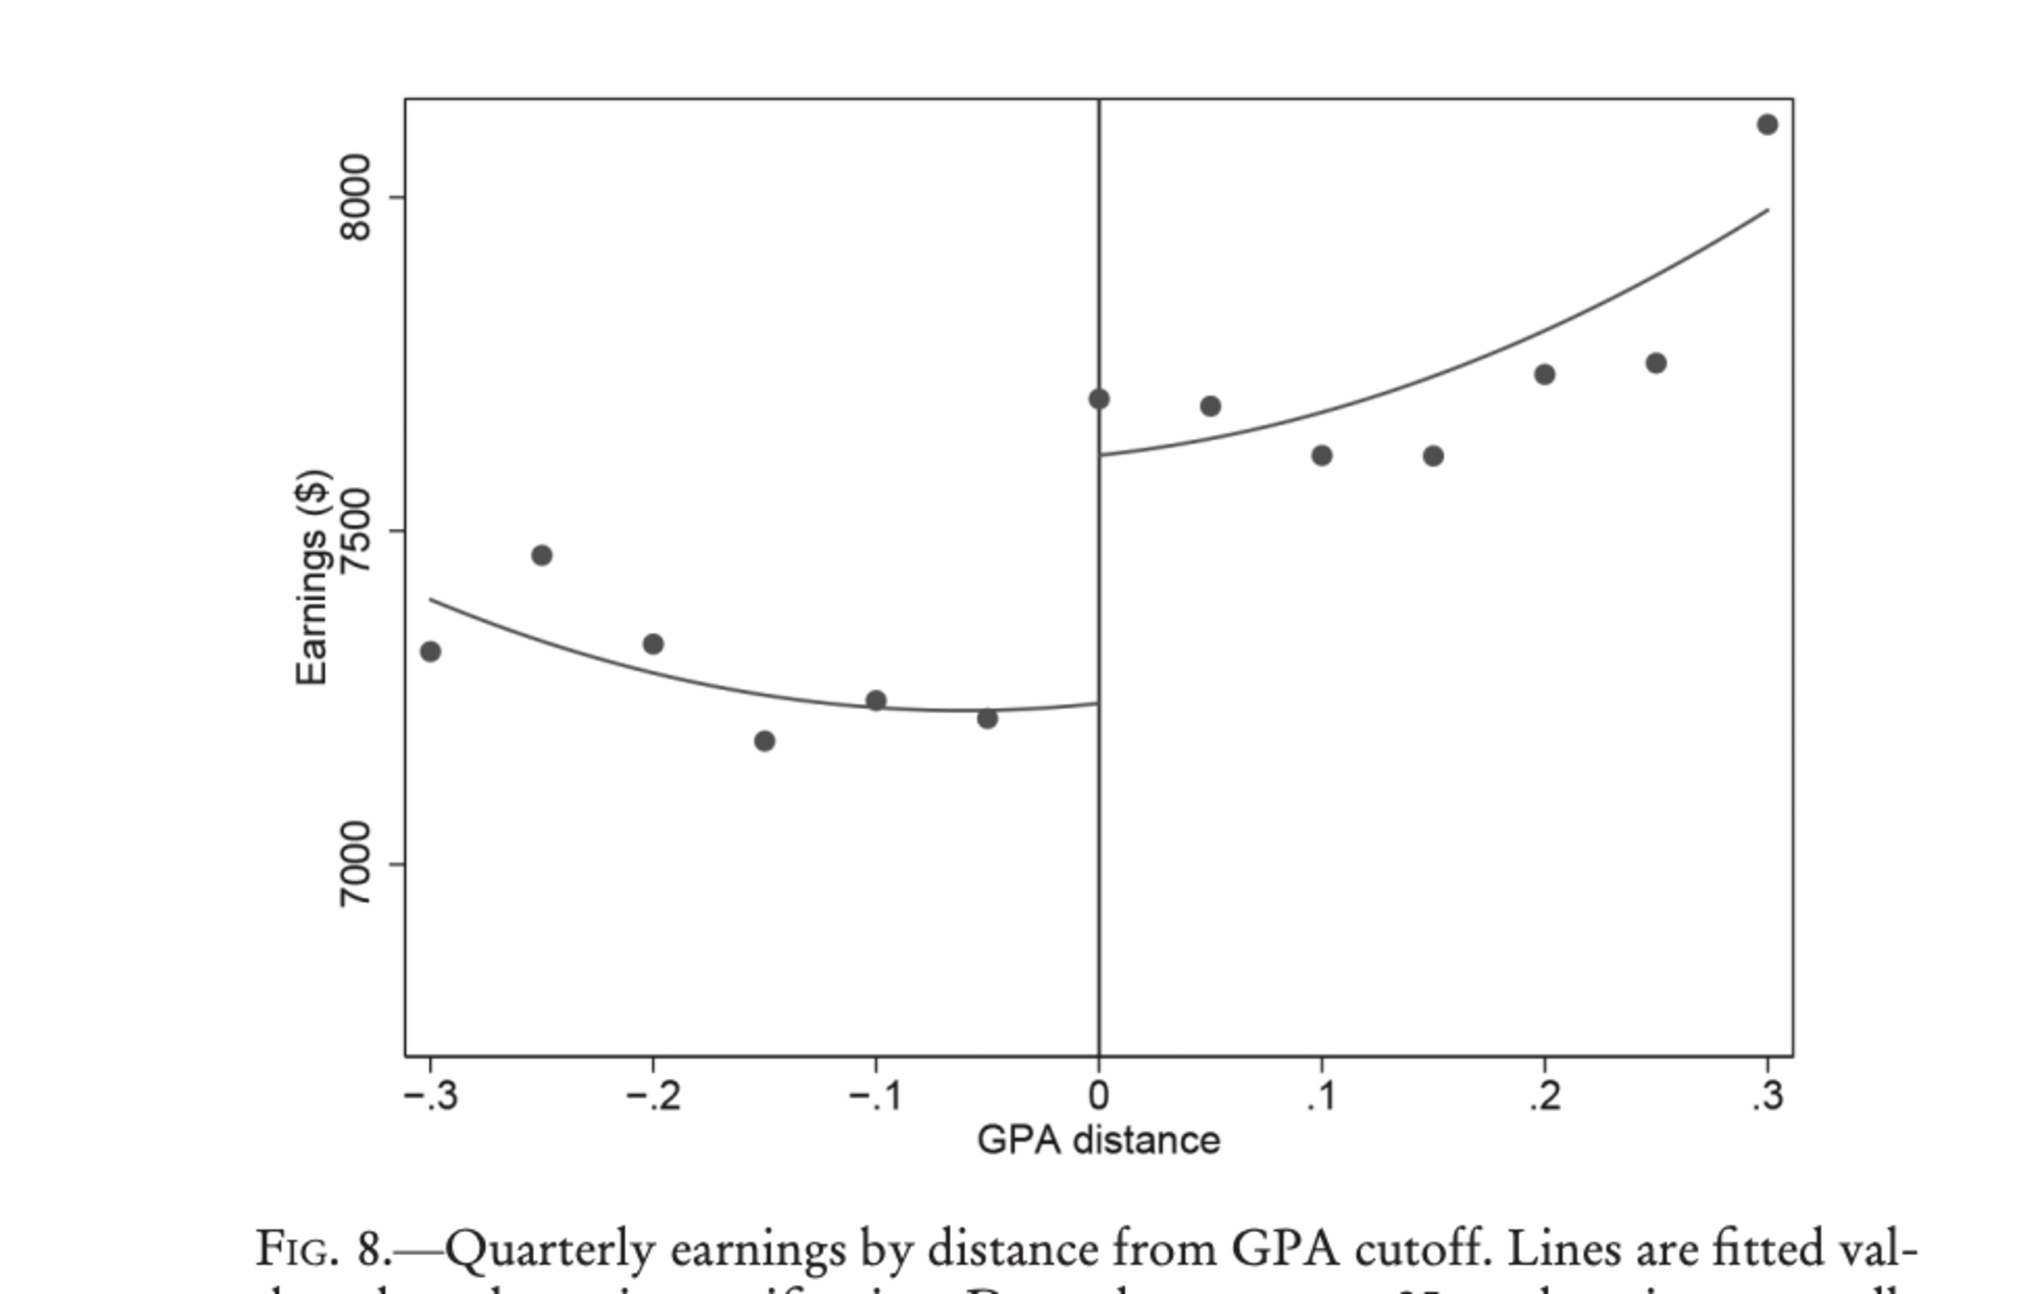
\includegraphics[width = 0.8\linewidth]{zimmerman-rf}
\end{frame}


\begin{frame}
	\centering
	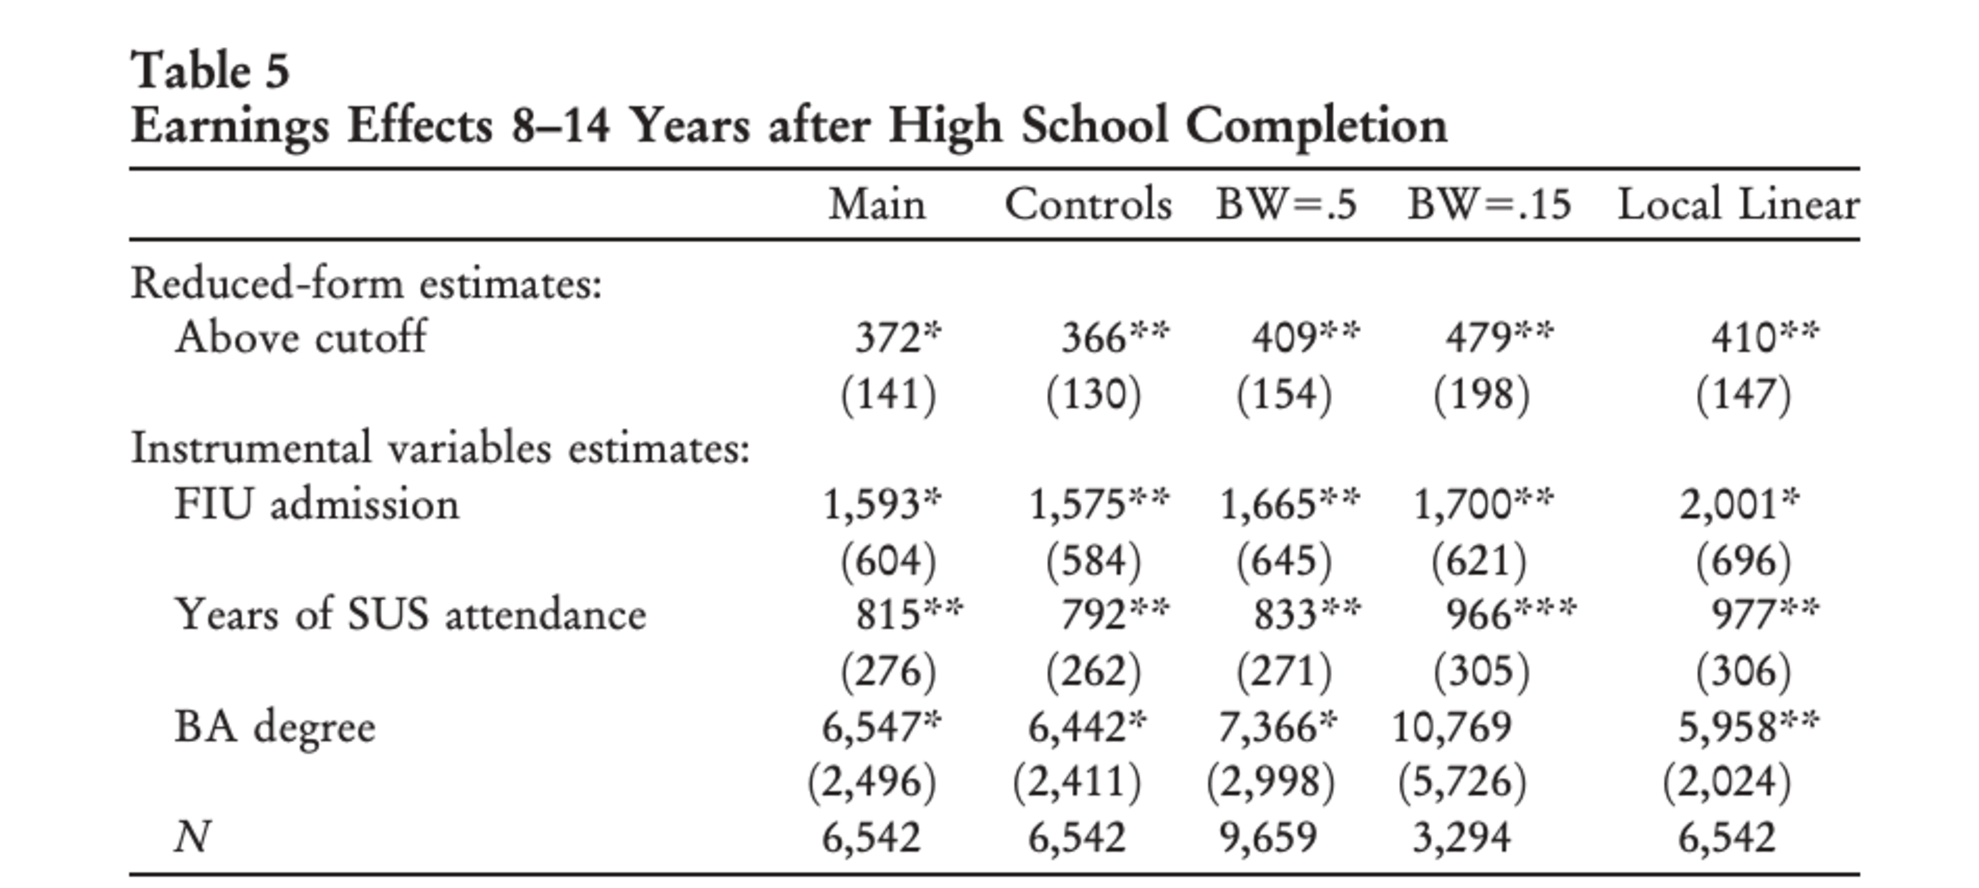
\includegraphics[width = 0.7\linewidth]{zimmerman-late} \\ 
	
	\begin{wideitemize}
		\item
		FIU への「入学（admission）」に対する第一段階と比較して、FIU への「進学（attendance）」に対する第一段階は約半分であることに注意してください。
		
		\item
		これは、進学の LATE が 3,000-4,000 ドル（カットオフ以下の平均所得の約半分）であることを示唆しています。
		
	\end{wideitemize}
	 
\end{frame}

\begin{frame}{議論}
	\begin{wideitemize}
		\item
		結果は、FIU に進学することの大きな収益を示唆しています。
		
		\item
		解釈における重要な問い：代替案は何でしょうか？ 
		
		\item
		論文は、コミュニティカレッジへの進学が減少していることを示しており、私立大学からの転換もあるかもしれません。
		
		\item
		底辺校の4年制公立大学におけるこの大きな収益は、「極めて選択度の高い大学」対「依然として選択度の高い大学」の差が小さいとした Dale \& Krueger の結果とは対照的です。
	\end{wideitemize}
\end{frame}


\end{document}
